\documentclass[12pt,a4paper]{article}
\usepackage[utf8]{inputenc}
\usepackage[brazil]{babel}
\usepackage{graphicx}
\usepackage{caption}
\usepackage{siunitx}
\usepackage{setspace}
\usepackage{float}
\usepackage[a4paper]{geometry}
\usepackage{amsmath,amsfonts,amstext,amscd,bezier}
\usepackage{mathtools}
\usepackage{amsthm}
\usepackage{mathrsfs}
\usepackage{times}
\usepackage{indentfirst}
\usepackage{hyperref}
\usepackage{placeins}
\usepackage{array}
\usepackage{subfigure}
\usepackage{wrapfig}
\usepackage{setspace}
\usepackage{gensymb}
\usepackage{svg}
\usepackage[backend=bibtex,sorting=none]{biblatex}
\usepackage{verbatim}
\usepackage[autostyle]{csquotes}
\usepackage{minted}
\linespread{1.1}

\begin{document}
	\begin{titlepage}
		\begin{center}
			\large Universidade de São Paulo\\[0.2cm]
			\large Instituto de Física de São Carlos\\[7cm]
			\huge \textbf{Relatório 2 - IntroFisComp}\\[6cm]
			
			\large Alexandre de Taunay Voloch \\[0.2cm]
		\end{center}
	\end{titlepage}

\section{Tarefa 1}

Aqui, apenas geramos números aleatórios utilizando o rand, e calculamos o momento de acordo com a fórmula dada.

\begin{minted}[
	mathescape,
	linenos,
	fontsize=\footnotesize,
	framesep=2mm,
	breaklines]
	{fortranfixed}
      implicit real*8 (a-h,o-z)
      parameter(N_iteracoes=10000000)

      somatotal = 0.e0

      write(*,*)"Insira n"
      read(*,*)n

      do i=1,N_iteracoes
         x = rand()
         somatotal = somatotal + (x**n)
      end do

      xmedio = somatotal / real(N_iteracoes)
      write(*,*)"<x^n>:", xmedio

      end


\end{minted}

Os resultados obtidos são:

\begin{minted}[
	mathescape,
	linenos,
	fontsize=\footnotesize,
	framesep=2mm,
	breaklines]
	{sh}
alex@G3-3590:~/projetos-fiscomp/projeto-2/tarefa-1$ ./tarefa-1.exe 
 Insira n
1
 <x^n>:  0.50001852986319062     
alex@G3-3590:~/projetos-fiscomp/projeto-2/tarefa-1$ ./tarefa-1.exe 
 Insira n
2
 <x^n>:  0.33333844544657659     
alex@G3-3590:~/projetos-fiscomp/projeto-2/tarefa-1$ ./tarefa-1.exe 
 Insira n
3
 <x^n>:  0.24999919177134661     
alex@G3-3590:~/projetos-fiscomp/projeto-2/tarefa-1$ ./tarefa-1.exe 
 Insira n
4
 <x^n>:  0.19999489197035913  
\end{minted}

Podemos ver, portanto, que de acordo com o programa rodado, podemos aproximar os momentos dessa distribuição como sendo:
$\langle x\rangle =0.5; \langle x^2\rangle =0.333; \langle x^3\rangle =0.25; \langle x^4\rangle =0.20$. 

Como podemos verificar isso experimentalmente? Como a função $rand()$ do Fortran gera números aleatórios distribuídos de forma uniforme no intervalo (0,1), então podemos calcular os seus momentos respectivos utilizando a fórmula

\[ \langle x^n\rangle  = \int_{0}^{1}x^n\rho_x(x)dx \]

Mas como temos uma distribuição uniforme de 0 a 1, $\rho_x(x) = 1$. Portanto temos
\[ \langle x^n\rangle  = \int_{0}^{1}x^ndx \]

Logo,
\[ \langle x\rangle  = \int_{0}^{1}xdx = \frac{1}{2} = 0.5 \]
\[ \langle x^2\rangle  = \int_{0}^{1}x^2dx = \frac{1}{3} = 0.333... \]
\[ \langle x^3\rangle  = \int_{0}^{1}x^3dx = \frac{1}{4} = 0.25\]
\[ \langle x^4\rangle  = \int_{0}^{1}x^4dx = \frac{1}{5} = 0.20\]

O que confirma nossos resultados obtidos pelo programa.

\section{Tarefa 2}
\subsection{a}

Nesse caso, precisamos gerar andarilhos aleatórios com probabilidade igual de ir para qualquer um dos dois lados. Fazemos isso sem utilizar um if com um algoritmo simples de conversão de número real para inteiro. Acabamos com um número que será ou 1 ou -1, e aí somamos isso na posição do andarilho respectivo. Também calculamos o primeiro e segundo momento e imprimimos ele ao final da execução.

\begin{minted}[
	mathescape,
	linenos,
	fontsize=\footnotesize,
	framesep=2mm,
	breaklines]
	{fortranfixed}
      implicit real*8 (a-h,o-z)
      parameter(m=1000000)
      parameter(n=1000)

      soma_x = 0.0
      soma_x2 = 0.0

      open(unit=1, file='tarefa-2a-saida.dat')

      do i=1,m
         ix_andarilho = 0
         do j=1,n
            irand = 2*int(2.e0 * rand()) - 1
            ix_andarilho = ix_andarilho + irand
         end do
         !write(*,*)ix_andarilho
         write(1,*)ix_andarilho

         soma_x = soma_x + real(ix_andarilho)
         soma_x2 = soma_x2 + real(ix_andarilho**2)

      end do

      close(1)
      soma_x = soma_x / real(m)
      soma_x2 = soma_x2 / real(m)

      write(*,*)"<x>:", soma_x
      write(*,*)"<x2>:", soma_x2

      end
\end{minted}

Na execução do programa acima, de 1000 passos para 1 milhão de andarilhos, obtemos:

\begin{minted}[
	mathescape,
	linenos,
	fontsize=\footnotesize,
	framesep=2mm,
	breaklines]
	{sh}
 <x>:  -4.3999999999999999E-005
 <x2>:   999.61015999999995     
\end{minted}

Ou seja, $\langle x\rangle  \approx 0$ e $\langle x^2\rangle  \approx 1000$. Esses resultados fazem sentido - como $p = q$, o andarilho tem probabilidade igual de andar para a direita ou para a esquerda e, portanto, deverá ter posição média na origem. Já o segundo momento central (é central pois $\langle x\rangle =0$) é dado pela fórmula no projeto

\[ \sigma_x^2 = 4a^2pqN = 4\frac{1}{4}1000 = 1000 \]

Plotando a distribuição num histograma, temos:

\begin{figure}[H]
\centering
\includegraphics[width=\linewidth]{../tarefa-2a/tarefa-2a.png}
\caption{Histograma dos andarilhos aleatórios com $p = q = 1/2$.}
\end{figure}

\subsection{b}
Nesse caso, precisamos de um algoritmo um pouco mais sofisticado para gerarmos o número da direção, considerando que $p \neq q$. Isso está feito no código abaixo. Basicamente, cria-se um número aleatório $0 < r < 1$. Definimos uma nova variável $x = p - r$, e pegamos o valor de $ix = \frac{x}{|x|}$, que será ou $+1$ ou $-1$. Note que, se $r>p$, então $ix = -1$, que corresponde (corretamente) a um passo à esquerda, e vice-versa para um passo para a direita.

Para gerar $\langle x\rangle , \langle x^2\rangle  e \sigma_x^2$ o procedimento é o mesmo que na tarefa anterior, exceto que no terceiro caso precisamos subtrair $\langle x\rangle $ de cada uma das iterações para conseguir o momento central, pois

\[ \sigma_x^2 = \langle  (x-\langle x\rangle )^2 \rangle  \]

O código é o seguinte:

\begin{minted}[
	mathescape,
	linenos,
	fontsize=\footnotesize,
	framesep=2mm,
	breaklines]
	{fortranfixed}
      implicit real*8 (a-h,o-z)
      parameter(m=1000000)
      parameter(n=1000)
      integer*16 iposicoes(m)
      integer*16 ix_andarilho

      soma_x = 0.d0
      soma_x2 = 0.d0
      soma_x2_central = 0.d0

      open(unit=1, file='tarefa-2b-saida.dat')

      write(*,*) "insira o denominador de p em forma real"
      read(*,*)denom
      p = 1.e0/denom

      do i=1,m
         iposicoes(i) = 0_16
         ix_andarilho = 0_16
         do j=1,n
            ! O algoritmo é o seguinte: para não termos que usar if, criamos uma nova variável x = p - r.
            ! Note que x < 0 caso r > p, que corresponde a um passo à esquerda com probabilidade 1 - p = q
            ! E que x > 0 caso r < p, que tem probabilidade p
            ! Depois para pegar -1 ou +1, fazemos x/|x|
            r = rand()
            x = p - r
            ix = int(x/abs(x), 16)

            ix_andarilho = ix_andarilho + ix
         end do
         write(1,*)ix_andarilho
         !write(*,*)ix_andarilho

         iposicoes(i) = ix_andarilho

      end do

      close(1)

      do i=1,m
         ! calcular <x>
         soma_x = soma_x + real(iposicoes(i))
      end do
      soma_x = soma_x / real(m)

      do i=1,m
         ! calcular <x^2> e a disperção central sigma^2
         soma_x2 = soma_x2 + real(iposicoes(i)**2)
         soma_x2_central = soma_x2_central + ( (real(iposicoes(i))
     &   - soma_x)**2.e0)
      end do

      soma_x2 = soma_x2 / real(m)
      soma_x2_central = soma_x2_central / real(m)

      write(*,*)"<x>:", soma_x
      write(*,*)"<x2>:", soma_x2
      write(*,*)"<x2> central:", soma_x2_central

      end

\end{minted}

Exemplos de execução:

\begin{minted}[
	mathescape,
	linenos,
	fontsize=\footnotesize,
	framesep=2mm,
	breaklines]
	{sh}
alex@G3-3590:~/projetos-fiscomp/projeto-2/tarefa-2b$ ./tarefa-2b.exe 
 insira o denominador de p em forma real
3.e0
 <x>:  -333.33947200000000     
 <x2>:   112003.78639199999     
 <x2> central:   888.58279876126892     
alex@G3-3590:~/projetos-fiscomp/projeto-2/tarefa-2b$ ./tarefa-2b.exe 
 insira o denominador de p em forma real
4.e0
 <x>:  -500.02133500000002     
 <x2>:   250769.69089699999     
 <x2> central:   748.35544181819262     
alex@G3-3590:~/projetos-fiscomp/projeto-2/tarefa-2b$ ./tarefa-2b.exe 
 insira o denominador de p em forma real
5.e0
 <x>:  -600.02238999999997     
 <x2>:   360666.45021200000     
 <x2> central:   639.58171068821594     

\end{minted}

Podemos estimar quanto deveriam ser os valores de $\langle x\rangle $, $\langle x^2\rangle $ e $\sigma_x^2$. De acordo com o projeto, temos

\[ \langle x\rangle  = a(2\langle n_d\rangle  - N) = a(2pN - N) = aN(2p -1)\]
\[ \langle x^2\rangle  = 4pN(pN+q) - 4pN^2 + N^2 \]
\[ \sigma_x^2 = 4pqN \]

Aplicando isso para $p = 1/3, 1/4, 1/5$ temos:

$p = 1/3$: $\langle x\rangle  = -333,333; \langle x^2\rangle  = 112000; \sigma_x^2 = 888,888$

$p = 1/4$: $\langle x\rangle  = -500; \langle x^2\rangle  = 250750; \sigma_x^2 = 750$

$p = 1/3$: $\langle x\rangle  = -600; \langle x^2\rangle  = 360640; \sigma_x^2 = 640$

Os valores acima são confirmados pelos valores calculados no programa.

Plotando os valores dessas três distribuições num gráfico, obtemos:

\begin{figure}[H]
\centering
\includegraphics[width=\linewidth]{../tarefa-2b/graficofull.png}
\caption{Histograma dos andarilhos aleatórios para diferentes valores de $p$.}
\end{figure}

\section{Tarefa 3}

Aqui, o programa é bem parecido com o da tarefa 2a, mas neste caso o andarilho está em duas dimensões, com igual probabilidade de andar em qualquer uma delas. O programa é o seguinte:

\begin{minted}[
	mathescape,
	linenos,
	fontsize=\footnotesize,
	framesep=2mm,
	breaklines]
	{fortranfixed}
      implicit real*8 (a-h,o-z)
      parameter(n_andarilhos=2000)
      integer iposicao(2)
      real*8 soma_r(2)

      soma_r(1)=0.0
      soma_r(2)=0.0
      soma_r2 = 0.0

      write(*,*)"Insira a potência de n (10^potência)"
      read(*,*)npot

      open(unit=1, file='tarefa-3-saida.dat')

      n = 10**npot

      do i=1,n_andarilhos
         iposicao(1) = 0
         iposicao(2) = 0
         do j=1,n
            ! como queremos 4 possibilidades, com 0.25 de chance cada um, fazemos o seguinte:
            ! primeiro escolhemos qual das direções (x ou y) iremos andar,
            ! depois fazemos outro rand() para decidir se vamos +1 ou -1 naquela direção

            idir = int(2*rand()) + 1 ! será ou 1 ou 2

            ! para decidir +1 ou -1 usamos o algoritmo da tarefa 2
            irand = 2*int(2.e0 * rand()) - 1

            !write(*,*) idir, irand

            iposicao(idir) = iposicao(idir) + irand
         end do
         !write(*,*)iposicao
         write(1,*)iposicao

         soma_r = soma_r + real(iposicao)
         soma_r2 = soma_r2 + real( (iposicao(1)**2) + (iposicao(2)**2) )

      end do
      close(1)

      soma_r = soma_r / real(n_andarilhos)
      soma_r2 = soma_r2 / real(n_andarilhos)

      write(*,*)"<r>:", soma_r
      write(*,*)"<r^2>:", soma_r2

      end

\end{minted}

Para $n=10^4$, temos

\begin{minted}[
	mathescape,
	linenos,
	fontsize=\footnotesize,
	framesep=2mm,
	breaklines]
	{sh}
 <r>: -0.59350000000000003       -1.2055000000000000     
 <r^2>:   9811.9609999999993   
\end{minted}

E, para $n=10^6$,

\begin{minted}[
	mathescape,
	linenos,
	fontsize=\footnotesize,
	framesep=2mm,
	breaklines]
	{sh}
<r>:  -38.618000000000002        17.184000000000001     
<r^2>:   1007217.8240000000    
\end{minted}

Perceba que $\langle r^2\rangle $ é aproximadamente igual a $n$, que é o comportamento esperado. Além disso, esperamos que $\langle \vec{r}\rangle  \approx (0,0)$. Podemos ver que isso é aproximadamente válido, porém, conforme o número de passos vai aumentando, como não temos tantos andarilhos (apenas 2000), ele se distancia do 0. Para testar, modifiquei o programa para 20000 andarilhos e $n=10^5$ passos, que nos fornece

\begin{minted}[
	mathescape,
	linenos,
	fontsize=\footnotesize,
	framesep=2mm,
	breaklines]
	{sh}
 <r>:  -3.9292899999999999        2.1856300000000002     
 <r^2>:   100223.04918000000     
\end{minted}

Que é um valor muito mais próximo à origem.

Como temos que $\langle \vec{r}\rangle  \approx (0,0)$, então o valor de $\Delta^2 = \langle \vec{r}\cdot\vec{r}\rangle  - \langle \vec{r}\rangle \cdot\langle \vec{r}\rangle $ é a mesma coisa que $\langle r^2\rangle  = n$ (o termos sendo subtraído é igual a 0, logo sobra apenas o módulo ao quadrado de $\vec{r}$).

Plotando todas as simulações num gráfico, obtemos

\begin{figure}[H]
\centering
\includegraphics[width=0.8\linewidth]{../tarefa-3/grafico.png}
\caption{Posição final dos andarilhos aleatórios em 2d, até $10^5$ passos}
\end{figure}

\begin{figure}[H]
\centering
\includegraphics[width=0.8\linewidth]{../tarefa-3/grafico2.png}
\caption{Posição final dos andarilhos aleatórios em 2d, até $10^6$ passos}
\end{figure}

\section{Tarefa 4}
Neste caso, utilizamos o código do exercício anterior para gerar andarilhos aleatórios, mas particionamos a geração de andarilhos em 2500 iterações, chegando, ao final, a $n$ passos. As iterações servem simplesmente para podermos calcular a entropia ao final de cada uma delas e gerar um gráfico da evolução da entropia ao longo do tempo (dos passos). 

Para calcular a entropia do sistema, dividimos o espaço em uma malha com reticulados de um tamanho muito maior do que o tamanho de um passo (1). Verificamos se há um andarilho dentro de cada uma dessas malhas e utilizamos isso para calcular a probabilidade de haver um andarilho na malha. Com isso, calculamos a entropia.

Segue o programa:

\begin{minted}[
	mathescape,
	linenos,
	fontsize=\footnotesize,
	framesep=2mm,
	breaklines]
	{fortranfixed}
      implicit real*8 (a-h,o-z)
      parameter(n_andarilhos=500) ! número de andarilhos
      parameter(itamanho_malha=3000) ! tamanho total da malha
      parameter(itamanho_particao=300) ! tamanho da subdivisão da malha
      parameter(n_passos=1000000) ! 1 milhão de passos
      parameter(n_iteracoes=2500) ! número de iterações/subdivisões do random walk
      integer iposicoes(n_andarilhos, 2) ! Matriz posição de cada um dos andarilhos

      open(unit=1, file='tarefa-4-saida.dat')

      ! primeiro inicializar a matriz iposicoes
      do i=1,n_andarilhos
         iposicoes(i,1) = 0
         iposicoes(i,2) = 0
      end do

      incremento_passos = n_passos/n_iteracoes ! Quantos passos damos em cada iteração
      i_n_divisoes_malha = itamanho_malha/itamanho_particao ! Quantas subdivisões temos em cada eixo da malha

      do niter=1,n_iteracoes
         write(*,*) "Iteração", niter, "de", n_iteracoes
         do j=( (niter-1)*incremento_passos ),(niter*incremento_passos)
            do i=1,n_andarilhos
               ! O seguinte código copiado da tarefa 3.

               ! como queremos 4 possibilidades, com 0.25 de chance cada um, fazemos o seguinte:
               ! primeiro escolhemos qual das direções (x ou y) iremos andar,
               ! depois fazemos outro rand() para decidir se vamos +1 ou -1 naquela direção

               idir = int(2*rand()) + 1 ! será ou 1 ou 2

               ! para decidir +1 ou -1 usamos o algoritmo da tarefa 2
               irand = 2*int(2.e0 * rand()) - 1

               iposicoes(i,idir) = iposicoes(i,idir) + irand
            end do
         end do
         ! Agora precisamos calcular a ENTROPIA do sistema. para fazer isso, vamos subdividir o espaço
         ! em uma malha de partição itamanho_particao.
         ! O tamanho total da malha, será de -3000 até 3000 nas duas direções (x e y)
         ! (escolhemos isso com base no gráfico da tarefa 3.)
         entropia = 0.e0
         do i=-i_n_divisoes_malha,i_n_divisoes_malha-1
            do j=-i_n_divisoes_malha,i_n_divisoes_malha-1
               n_dentro = 0
               do k=1,n_andarilhos
                  ! como calculamos Pi? simplesmente vemos quantos andarilhos estão dentro dessa célula, e dividimos pelo número total
                  ! de andarilhos!
                  ! Como calcular se está dentro:
                  ! i*itamanho_particao <= x_adarilho < (i+1)*itamanho_particao
                  ! e o mesmo para y
                  ! j*itamanho_particao <= y_andarilho < (j+1)*itamanho_particao
                  ix_andarilho = iposicoes(k, 1)
                  iy_andarilho = iposicoes(k, 2)

                  if ( ((i*itamanho_particao).le.ix_andarilho).and.
     &            ( ((i+1)*itamanho_particao).gt.ix_andarilho ).and.
     &            ( (j*itamanho_particao).le.iy_andarilho).and.
     &            ( ((j+1)*itamanho_particao).gt.iy_andarilho )) then
                     n_dentro = n_dentro + 1
                  end if
               end do
               pi = real(n_dentro)/real(n_andarilhos)
               if(pi.gt.0.e0)then
                  entropia = entropia - (pi * log(pi))
                  write(*,*)"Encontramos", n_dentro,
     &            "andarilhos no ponto", i, j, "pi=", pi
               end if
            end do
         end do
         write(*,*)"Entropia:", entropia
         ! no arquivo, escrevemos o número N de passos no eixo x, e a entropia no eixo Y
         write(1,*)niter*incremento_passos,entropia

      end do

      close(1)

      end
\end{minted}

Para $n = 10^6$ passos, e variando o tamanho da partição, obtemos o seguinte gráfico:

\begin{figure}[H]
\centering
\includegraphics[width=\linewidth]{../tarefa-4/grafico.png}
\caption{Evolução da entropia dos andarilhos aleatórios em 2d ao longo do tempo.}
\end{figure}

Como podemos ver, as partições menores tendem assintoticamente a um valor específico, e saem do regime linear muito rapidamente, enquanto que partições maiores demoram para sair do regime linear. Todas as curvas têm formato logarítmico, que é o esperado para uma grandeza como a entropia (que é calculada de forma logarítmica.)

\end{document}